\documentclass{beamer}

\usepackage{graphicx}
\usepackage{caption}

\mode<presentation>
{
  \usetheme{Warsaw}

  \setbeamercovered{transparent}
}

\title{Gradient Coding}

\author{Runtian Zhu \\ \texttt{zhurt23@m.fudan.edu.cn}}

\date{2023.10.7}

\begin{document}

\captionsetup[figure]{labelformat=empty}

\begin{frame}
  \titlepage
\end{frame}

\begin{frame}{Outline}
  \tableofcontents
\end{frame}

\section{Gradient Coding}

\begin{frame}{References}

\begin{itemize}
    \item R. Tandon, Q. Lei, A. G. Dimakis, and N. Karampatziakis, “Gradient coding: Avoiding stragglers in distributed learning,” in International Conference on Machine Learning, PMLR, 2017, pp. 3368–3376.
\end{itemize}

\begin{figure}
    \centering
    \begin{minipage}[t]{.2\paperwidth}
        \centering
        
\includegraphics[width=\textwidth]{res/Rashish Tandon.jpg}
        \caption{Rashish Tandon}
    \end{minipage}
    \begin{minipage}[t]{.2\paperwidth}
        \centering
        
\includegraphics[width=\textwidth]{res/Qi Lei.jpg}
        \caption{Qi Lei}
    \end{minipage}
    \begin{minipage}[t]{.2\paperwidth}
        \centering
        
\includegraphics[width=\textwidth]{res/alexdimakis_sm.jpg}
        \caption{Alexandros G. Dimakis}
    \end{minipage}
    \begin{minipage}[t]{.2\paperwidth}
        \centering
        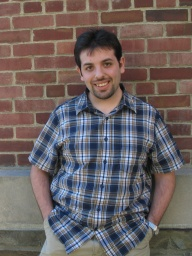
\includegraphics[width=\textwidth]{res/Nikos Karampatziakis.jpg}
        \caption{Nikos Karampatziakis}
    \end{minipage}
\end{figure}

\end{frame}

\begin{frame}{Background}{Distributed Learning}

\begin{figure}
    \centering
    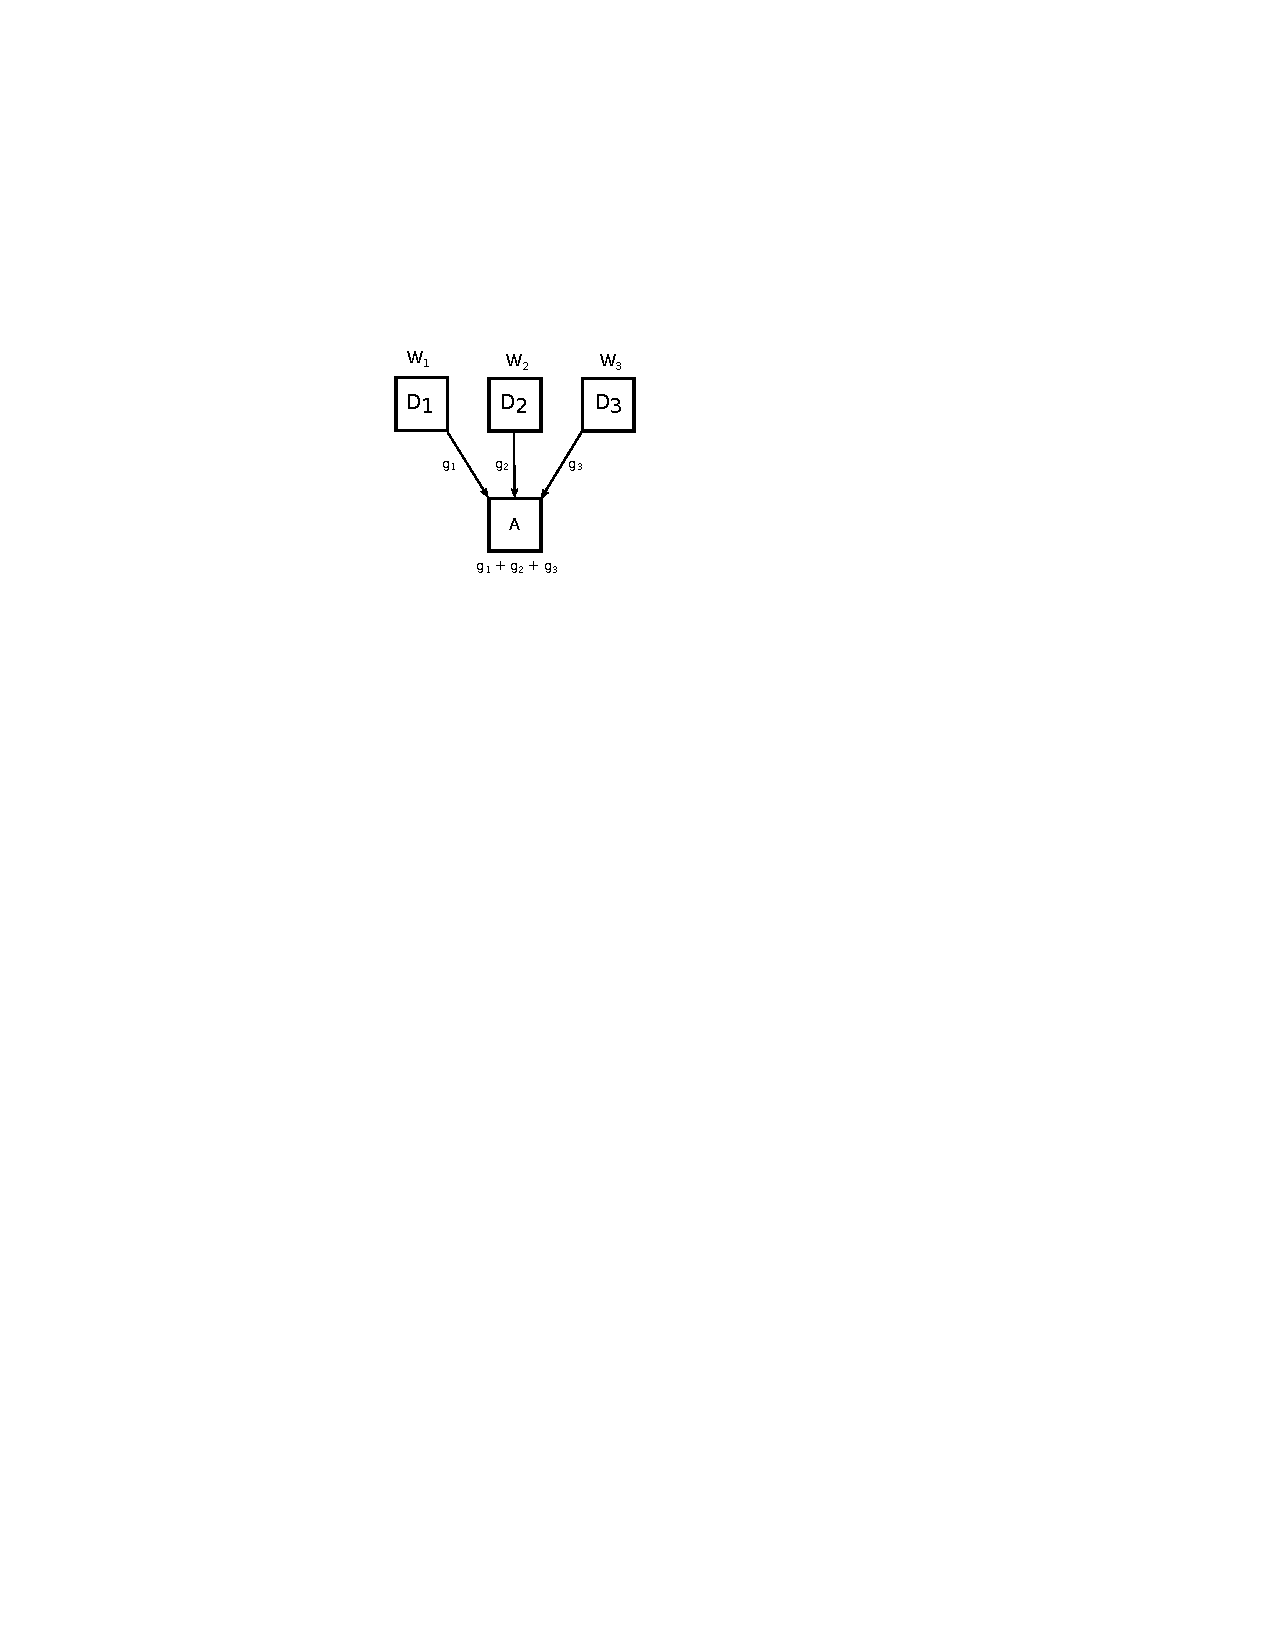
\includegraphics{res/distributed_learning.pdf}
\end{figure}

gradient descent

\end{frame}

\section{Further Work}

\subsection{DRACO}

\begin{frame}{DRACO}

\end{frame}

\subsection{Interactive Gradient Coding}

\begin{frame}{Interactive Gradient Coding}

\end{frame}

\end{document}

